\section{Математическая модель}

\begin{quotation}
Рассматриваемый механизм (рис. \ref{fig:scheme}) состоит из корпуса, внутри которого расположен эксцентриковый вал с маховиками на концах. На этом валу установлены эксцентриковые механизмы, каждый из которых состоит из двух эксцентриков, вставленных друг в друга с возможностью изменения положения шайб, что позволяет регулировать величины эксцентриситетов $r_i$ и сдвигов по фазам $\varphi_i$ между ними ($i={1,2,3,...,N}$). На свободных концах шатунов установлены шарнирно поршни-ударники. Эксцентриковые механизмы вместе с шатунами и поршнями-ударниками преобразуют вращательное движение вала с постоянной циклической частотой вращения маховика $\omega$ в возвратно-поступательное движение корпуса относительно стоек. ПУ расположены один внутри другого и ударяются каждый по своей наковальне высоты $h_i$.
\end{quotation}

\begin{figure}[H]
    \centering
    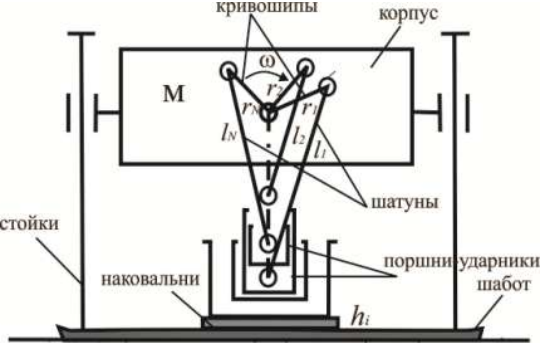
\includegraphics[width=0.6\textwidth]{../imgs/scheme.png}
    \caption{\parbox{0.6\textwidth}{Схема ударно-вибрационного механизма с кривошипношатунным возбудителем колебаний.}}
    \label{fig:scheme}
\end{figure}

\centering\subsection{Размерный вид}

\begin{quotation}
Колебания корпуса совершаются относительно того механизма, сумма
проекций геометрических размеров на вертикальную ось которого в данный
момент наибольшая.
Удар о наковальню одновременно одного или
нескольких ПУ происходит либо при смене взаимодействующих с
наковальней ПУ, либо после отрыва корпуса вместе с эксцентриковыми
механизмами.

Пренебрегая массами ПУ, шатунов и кривошипов, уравнение
свободного движения системы при $y_{pi} > 0$ может быть записано в виде
\end{quotation}

\Large\centering
$M\frac{{d^2 y}}{{d t^2}} = -Mg$\\[5mm]
\normalsize

\begin{quotation}
y - координата центра масс корпуса, отсчитываемая от наковальни,
$y_{pi}$ - величины, характеризующие отклонение оснований i - ого ПУ,
g - ускорение силы тяжести.

При соприкосновении одного из ПУ с наковальней $y_{pi} = 0$
происходит мгновенное ударное взаимодействие, такое, что если $\dot{y}_{pi}^-$ и $\dot{y}_{pi}^+$
скорости i-го ПУ непосредственно до и после ударного взаимодействия
соответственно, то
\end{quotation}

\Large\centering
$\dot{y}_{pi}^+ = -R\dot{y}_{pi}^-$
\normalsize

\begin{quotation}
Положение эксцентриситетов длиной $r_i$
будем измерять углами $\omega t - \varphi$
отсчитываемые от вертикальной оси (рис. \ref{fig:geometric-diagram}).
Тогда можно вывести соотношение:
\end{quotation}

\Large
$y_{pi} = y - s_i + r_i \cos(\omega t - \varphi_i) - \sqrt{l_i^2 - r_i^2 \cos(\omega t - \varphi_i)}$
\normalsize 

\begin{figure}[H]
    \centering
    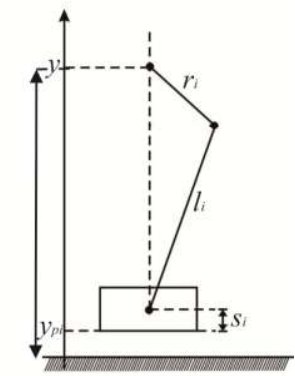
\includegraphics[height=0.3\textheight]{../imgs/geometric-diagram.png}
    \caption{\parbox{0.25\textwidth}{Геометрическая схема.}}
    \label{fig:geometric-diagram}
\end{figure}


Получаем уравнения движения механизма в размерном виде:
\Large
\begin{align*}
\left\{
\begin{array}{ll}
\left\{
\begin{array}{l}
y_{pi} > 0 \\
M \frac{d^2 y}{dt^2} = -Mg
\end{array}
\right. & \\[2mm]
\left\{
\begin{array}{l}
y_{pi} = 0 \\
\dot{y}_{pi}^+ = -R \dot{y}_{pi}^-
\end{array}
\right. & \\[2mm]
y_{pi} = y - s_i + r_i \cos(\omega t - \varphi_i) - \sqrt{l_i^2 - r_i^2 \cos(\omega t - \varphi_i)}
\end{array}
\right.
\end{align*}
\normalsize

\begin{quotation}
С учётом условия $r_i << l, l_i \approx l$ последнее уравнение будет: 

\centering$y_{pi} = y - s_i + r_i \cos(\omega t - \varphi_i) - l$
\end{quotation}

\subsection{Безразмерный вид}

\Large
$
\begin{cases}
\frac{{d^2 x}}{{d \tau^2}} = -p, & x > f(\tau) \\[2mm]
\frac{{dx}}{{d\tau}}|_+ = -R \frac{{dx}}{{d\tau}}|_- + (1 + R) \frac{{df(\tau)}}{{d\tau}}, & x = f(\tau), \quad \dot{x} - \frac{{df}}{{d\tau}} < 0
\end{cases}
$
\\[8mm]
\large
{
$
f(\tau) = \max\{f_1(\tau), f_2(\tau), ..., f_N(\tau)\},\quad f_i(\tau) = \mathcal{E}_i - \mu \gamma_i \cos(\tau - \varphi_i)
$
}
\normalsize